Im Rahmen dieser Arbeit wurden zwei Systeme zur Erkennung von Hindernissen in Echtzeit entwickelt. Diese richten sich nach den in Kapitel REF erläuterten Algorithmen und Konzepten. Anhand dieser ist es möglich aus den beiden Bildern des Stereo Systems für jeden Frame die Disparity Map zu berechnen, welche im Anschluss daran in mehreren Schritten zunächst so angepasst wird, dass nicht verwertbare Bereiche der Tiefenkarte entfernt werden (siehe REF preprocessing). Dies reduziert die Anzahl der zur Erkennung zu verarbeitenden Punkte und somit die Rechenzeit.\\

\noindent
Im folgenden Kapitel werden beide Methoden detailliert beleuchtet. Zu Beginn wird die zugrunde liegende Klassenstruktur beschrieben. In Abschnitt \ref{sec:mean_disparity_detection} die \emph{Mean Disparity Detection} erläutert, wobei auf das grundlegende Konzept sowie den Algorithmus zur Erkennung selber eingegangen wird. Selbiges gilt für die \emph{Samplepoint Detection} in Abschnitt \ref{sec:samplepoint_detection}.


%\begin{figure}[h]
%	\begin{center}
%	    %TODO: change Samplepoint Detection mImageCenter to private
%	    %TODO: add Subimage Stuff to MeanDisparityDetection
%		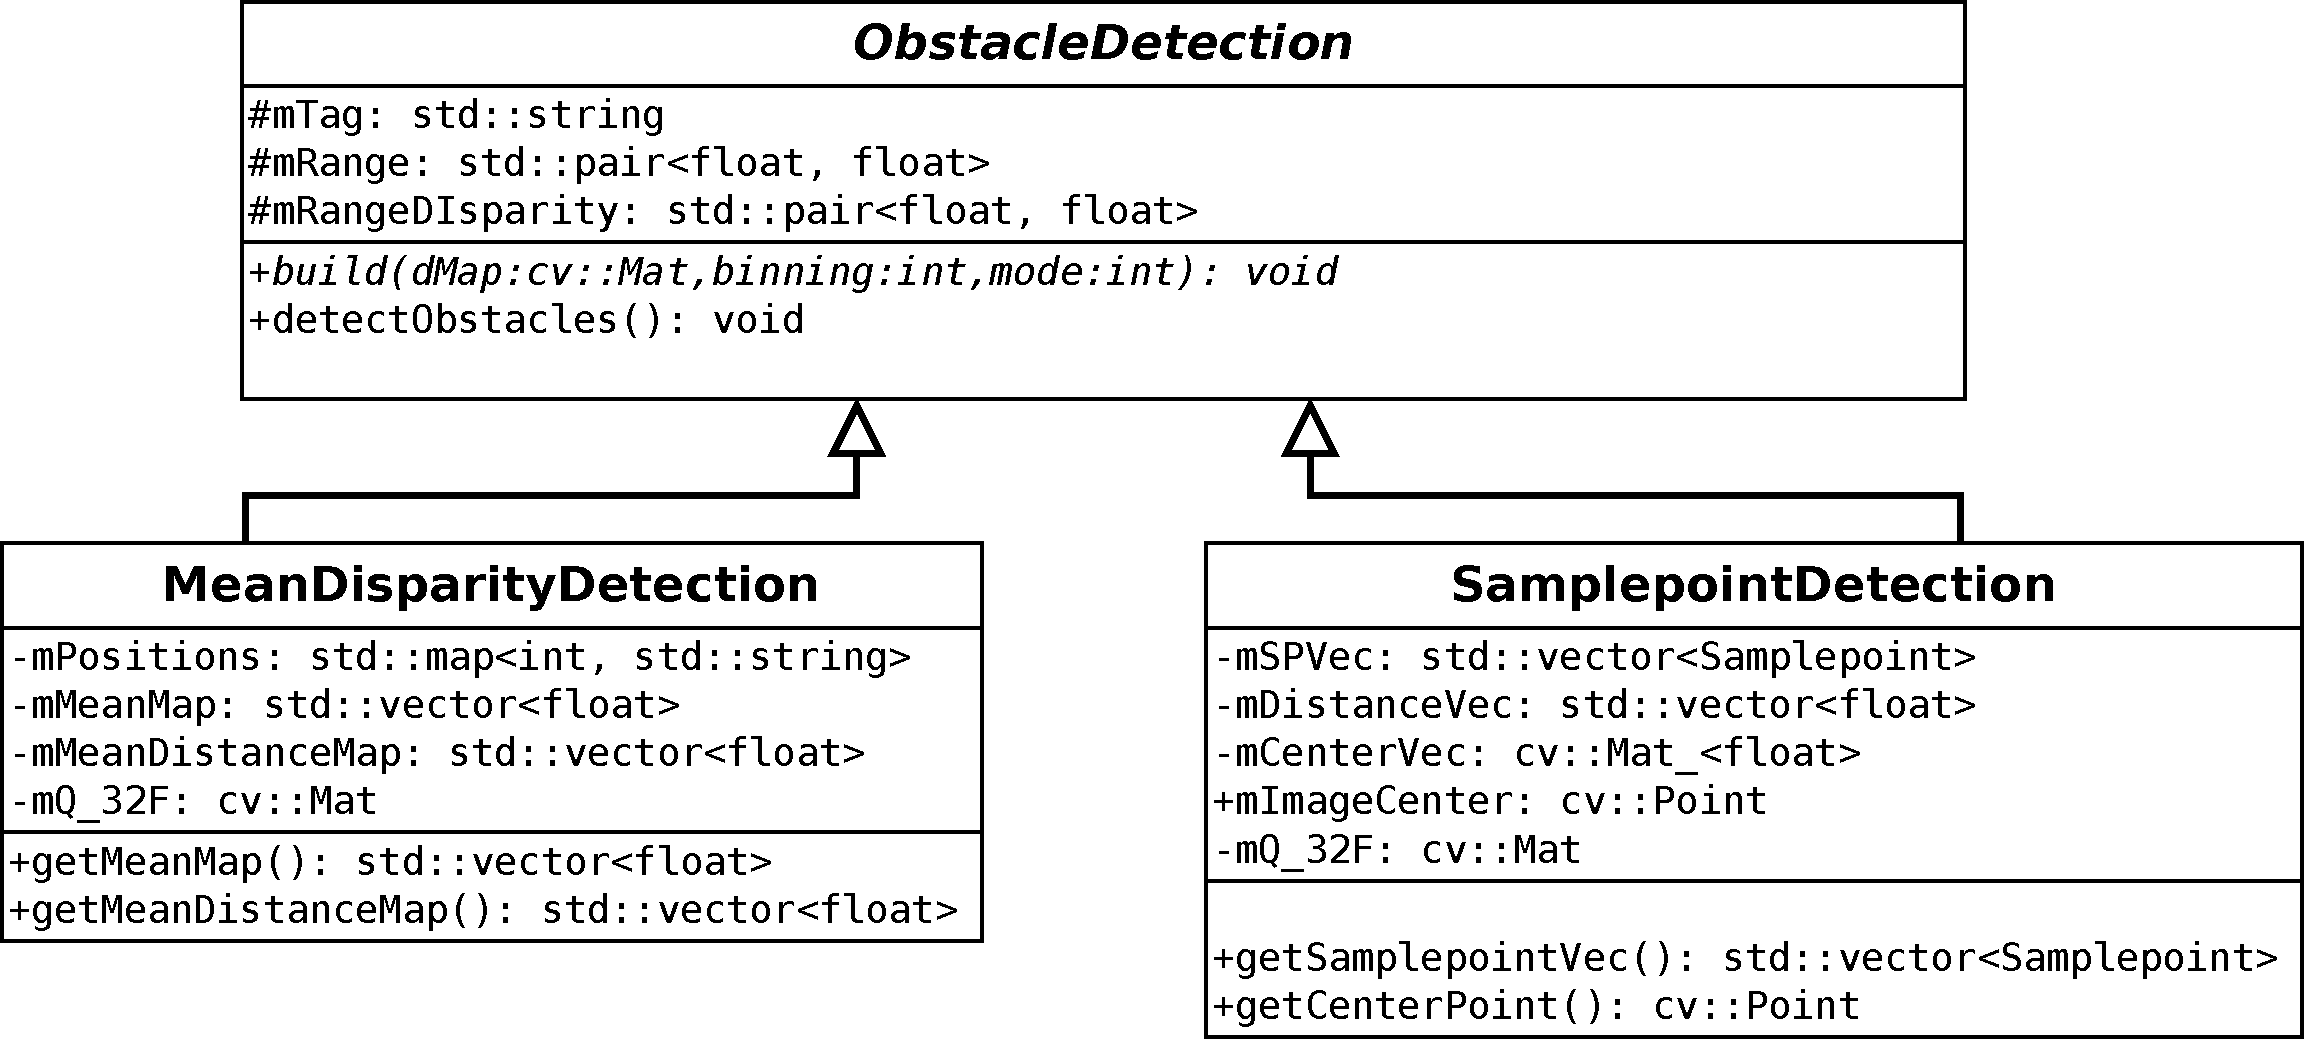
\includegraphics[width=13cm]{img/obstacle_detection_structure.pdf}
%	\end{center}
%	\caption{Klassenstruktur der Hinderniserkennung}
%	\label{fig:obstacle_detection_structure}
%\end{figure}



% ---------------------- section -----------------------
\section{Mean Disparity Detection}
\label{sec:mean_disparity_detection}

Das grundlegende Funktionsprinzip der \emph{Mean Disparity Detection} ist grob an die von Kostavelis et al. vorgestellten Algorithmen angelehnt. Auch bei diesen werden die berechneten Disparity Maps in Segmente eingeteilt von welchen in jedem Frame der Mittelwert errechnet wird.

Zu Beginn des Algorithmus, nach der vorherigen Bearbeitung der eigentlichen \emph{region of interest}, wird während der Initialisierung die Segmentierung der Disparity Map festgelegt. Dabei wird für jedes Segment ein eigenes Subimage erzeugt. Diese definieren eine \emph{region of interest} (ROI) innerhalb einer Matrix. Subimages selber halten lediglich die Positionsinformationen (obere linke und untere rechte Ecke des definierten Rechtecks), Mittelwert der ROI, die ROI selbst sowie den Mittelpunkt des Rechtecks zur späteren Pointcloud Generierung, wie Abbildung REF aufzeigt.

Für die Unterteilung der Disparity Map wurden intial nur 9 Segmente vorgesehen wobei jeder Bereich eine der möglichen Flugrichtungen repräsentieren sollte. Aufgrund der Größe der Submatrizen konnte jedoch keine valide Erkennung kleiner Hindernisse gewährleistet werden, da solche in der Berechnung des Mittelwertes untergegangen sind. Aufgrund dessen wurde die Anzahl der Segmente auf 81 erhöht, welches eine wesentlich genauere Erkennung ermöglicht. Zudem ist somit eine weitaus genauere Einteilung der Flugrichtungen möglich, da jede dieser nocheinmal genauer betrachtet wird (siehe Abbildung REF).

Um die Hindernisse innerhalb der Segmente zu Erkennen wurde auf die Berechnung des Mittelwertes gesetzt. Einerseits, da die Berechnung des Mittelwertes unter Betrachtung des Echtzeit-Aspektes eine ressourcensparende und schnelle Operation ist, andererseits weil jeder Pixel des Bildes in das Endresultat mit einfließt. Jedoch musste die Berechnung auf das Szenario angepasst werden, da Berechnung des Medians aller Werte zu Verzerrungen geführt hätte. Bei der Kalkulation von Disparity Maps werden Bereiche welche nicht gematcht werden können, sei es aufgrund von fehlenden Informationen im Referenzbild oder homogener Texturen in der Szene, als negativer Wert ausgedrückt. Berechnet man nun den Mittelwert unter Betrachtung positiver und negativer Werte, so entspricht dies zwar dem definierten Term Median, verfälscht allerdings das in diesem Anwendungsbereich erwünschte Ergebnis. Im schlechtesten Fall enthält eine Submatrix mehr negative als positive Werte, was dazu führen kann das Hindernisse vor homogenen Flächen nicht erkannt werden. Daraus ergibt sich die in Algorithmus \ref{alg:mean_disparity_calculation} dargestellte Berechnung des Mittelwertes.

\begin{algorithm}[h]
\caption{Berechnung des Disparity Medians}
\label{alg:mean_disparity_calculation}
\begin{algorithmic}[1]
    \Procedure{CalcMeanDisparity}{$submatrix$}
        \State $elements_{number} \gets 0$
        \State $elements_{sum} \gets 0 $
        \For{$value$ in $submatrix$}
            \If{$value > 0$}
                \State $elements_{sum} \gets elements_{sum} + value$
                \State $elements_{number} \gets elements_{number} + 1$
            \EndIf
        \EndFor
        \State \textbf{return} $elements_{sum} / elements_{number}$
    \EndProcedure
\end{algorithmic}  
\end{algorithm}

Es werden also nur positive Disparitäten betrachtet was auch dazu führt, dass sich der Gesamtwert aller Werte aus der Menge dieser ergibt. Mit Hilfe dieser Berechnung ist es möglich Hindernisse auch in Bereichen zu erkennen wo die Mehrzahl der Pixel keine Matches aufweisen.\\

\noindent
Die eigentliche Hinderniserkennung erfolgt in jedem Frame. Wobei der Term Frame hierbei nicht nach einem von der Kamera aufgenommenen Bild, sondern eine neue Disparity Map definiert. Da die Bildgröße pro Einzelbild stetig ist besteht keine Nötigkeit die einzelnen Segmente erneut zu generieren. Es genügt also die Mittelwerte eines jeden Subimages anhand der neuen Disparity Map zu aktualisieren. Daraufhin wird geprüft ob sich einer oder mehrere der Subimage Mittelwerte innerhalb der Gefahrenzone befinden. Anschließend wird unter Zuhilfenahme der neuen Werte eine Pointcloud erstellt und geloggt. Der gesamte Ablauf des der Hinderniserkennung wird in Algorithmus \ref{alg:mean_disparity_detection} dargestellt.\\

\begin{algorithm}[h]
\caption{Ablauf der Hinderniserkennung}
\label{alg:mean_disparity_detection}
\begin{algorithmic}[1]
    \Procedure{detectObstacles}{$submatrix$}
        \State $elements_{number} \gets 0$
        \State $elements_{sum} \gets 0 $
        \For{$value$ in $submatrix$}
            \If{$value > 0$}
                \State $elements_{sum} \gets elements_{sum} + value$
                \State $elements_{number} \gets elements_{number} + 1$
            \EndIf
        \EndFor
        \State \textbf{return} $elements_{sum} / elements_{number}$
    \EndProcedure
\end{algorithmic}  
\end{algorithm}

\noindent
Die in Algorithmus \ref{alg:mean_disparity_detection} berechnete Pointcloud ist in diesem Fall ein Matrix mit der Größe der ursprünglichen Tiefenkarte. Mithilfe der Mittelpunkte der Subimages wird für jedes dieser der jeweilige Tiefenwert an der Position des Mittelwertes abgelegt, dabei ist die Beibehaltung der ursprünglichen Größe für die Berechnung der Distanz (Formel \ref{eq:distance_calculation}) zum Hindernis von Nöten.

\begin{equation}\label{eq:distance_calculation}
    \begin{aligned}
        \begin{bmatrix}
            X\\ Y \\ Z\\ W
        \end{bmatrix}
        = Q \cdot 
        \begin{bmatrix}
            image_x\\ image_y \\ disparity(x,y)\\ 1
        \end{bmatrix}\\
        pointcloud(x,y) = [\frac{X}{W}, \frac{Y}{W}, \frac{Z}{W} ]
    \end{aligned}
\end{equation}

% ---------------------- section -----------------------
\section{Samplepoint Detection}
\label{sec:samplepoint_detection}

